
En ville, la vitesse est limitée à 50 $km.h^{-1}$. Le tableau ci-dessous indique les vitesses dépassant la limite autorisée lors d’un contrôle avec un radar.

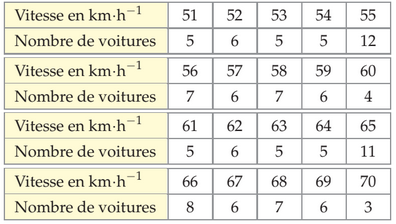
\includegraphics[scale=1]{stat-tableau.png} 

Dans un compte-rendu de ce contrôle, on peut lire : Un quart des automobilistes en infraction le sont pour une vitesse n'excédant pas de 5 $km.h^{-1}$ de la limite autorisée, la moitié des automobilistes en infraction n'excèdent pas la vitesse autorisée de plus de 10 $km.h^{-1}$, et 75 \% des automobilistes en infraction n'excèdent pas la vitesse autorisée de plus de 15 $km.h^{-1}$.

Que penser de ces affirmations ?